\documentclass[tikz,border=6pt]{standalone}
% Shared visual language for the book's standalone vector figures.
% Keep this file compatible with the TeX Live version used by LyX.
\usepackage{amsmath,amssymb}
\usepackage{array,booktabs}
\usepackage{pgfplots}
\usepackage{pgfplotstable}
\usetikzlibrary{arrows.meta,calc,positioning}
\pgfplotsset{compat=1.17}

\definecolor{BookBlue}{HTML}{0072B2}
\definecolor{BookOrange}{HTML}{D55E00}
\definecolor{BookGreen}{HTML}{009E73}
\definecolor{BookGray}{HTML}{666666}
\definecolor{BookLightGray}{HTML}{D9D9D9}

\pgfplotsset{
  book axis/.style={
    axis line style={black!75,line width=0.55pt},
    tick style={black!75,line width=0.45pt},
    tick label style={font=\small},
    label style={font=\small},
    legend style={
      font=\small,
      draw=none,
      fill=none,
      cells={anchor=west},
    },
    grid style={BookLightGray,line width=0.35pt},
    major grid style={BookLightGray,line width=0.35pt},
  },
}

\begin{document}
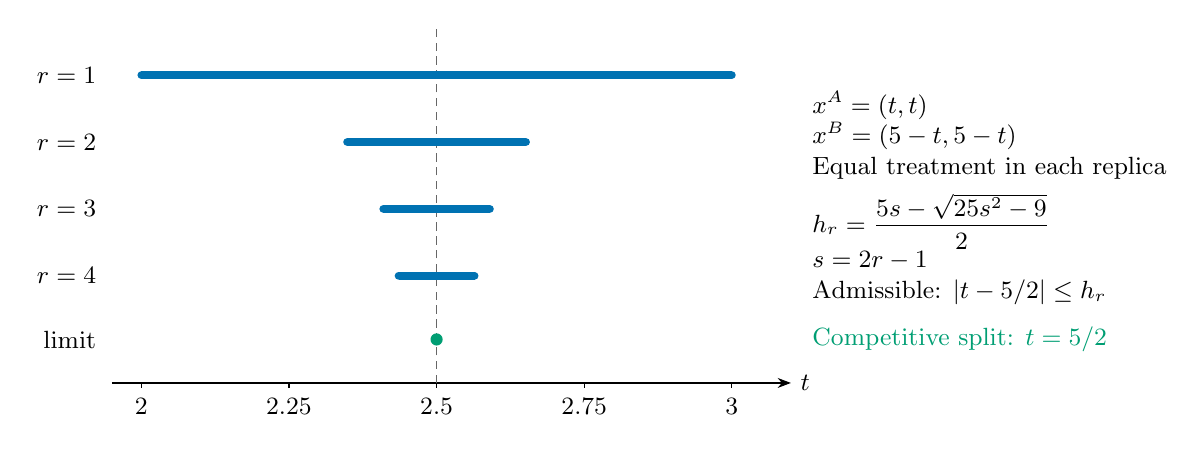
\begin{tikzpicture}[x=7.5cm,y=.85cm,>=Stealth,font=\small]
 \draw[->] (1.95,0)--(3.1,0) node[right] {$t$};
 \foreach \v in {2,2.25,2.5,2.75,3}
   {\draw (\v,0)--(\v,-.08) node[below] {$\v$};}
 \draw[BookGray,densely dashed] (2.5,0)--(2.5,5.3);
 \foreach \r/\y in {1/4.6,2/3.6,3/2.6,4/1.6}{
  \pgfmathsetmacro{\ss}{2*\r-1}
  \pgfmathsetmacro{\hh}{(5*\ss-sqrt(25*\ss*\ss-9))/2}
  \draw[BookBlue,line width=3pt] ({2.5-\hh},\y)--({2.5+\hh},\y);
  \fill[BookBlue] ({2.5-\hh},\y) circle(1.4pt);
  \fill[BookBlue] ({2.5+\hh},\y) circle(1.4pt);
  \node[anchor=east] at(1.94,\y){$r=\r$};
 }
 \fill[BookGreen] (2.5,.65) circle(2.2pt);
 \node[anchor=east] at(1.94,.65){limit};
 \node[anchor=west,align=left] at(3.12,3.7)
 {$x^A=(t,t)$\\$x^B=(5-t,5-t)$\\Equal treatment in each replica};
 \node[anchor=west,align=left] at(3.12,2)
 {$h_r=\dfrac{5s-\sqrt{25s^2-9}}2$\\$s=2r-1$\\Admissible: $|t-5/2|\leq h_r$};
 \node[anchor=west,BookGreen] at(3.12,.65){Competitive split: $t=5/2$};
\end{tikzpicture}
\end{document}
